\nsection{Turtle Graphics}

\subsection*{History}
\begin{itemize}
\item Many attempts have been made to create programming languages
which are intuitive and easy to learn.
\item One of the best of these was {\it LOGO} which allowed
children as young as 3 to learn a computer language.
\item A subset of this language involved a ``turtle'' which
could be driven around the screen using simple instructions.
The turtle, when viewed from above, was represented by a triangle.
\end{itemize}

\subsection*{An Example}
\begin{codesnippet}
{
 FD 30
 LT 45
 FD 30
 LT 45
 FD 30
 LT 45
 FD 30
 LT 45
 FD 30
 LT 45
 FD 30
 LT 45
 FD 30
 LT 45
 FD 30
 LT 45
}
\end{codesnippet}
\begin{center}
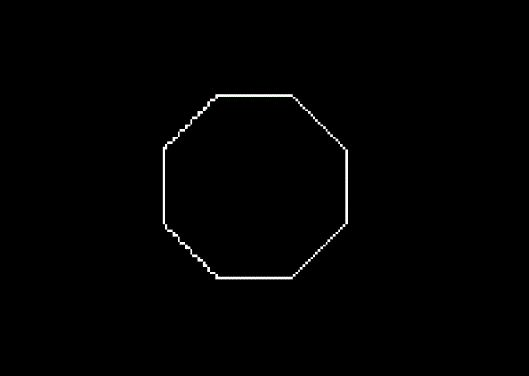
\includegraphics[width=4in]{../Pictures/octagon.jpg}
\end{center}


\subsection*{Adding Loops}
\begin{codesnippet}
{
   DO A FROM 1 TO 8 {
      FD 30
      LT 45
   }
}
\end{codesnippet}

\subsection*{Using Variables}
\begin{codesnippet}
{
   DO A FROM 1 TO 100 {
      SET C := A 1.5 * ;
      FD C
      RT 62
   }
}
\end{codesnippet}
\begin{center}
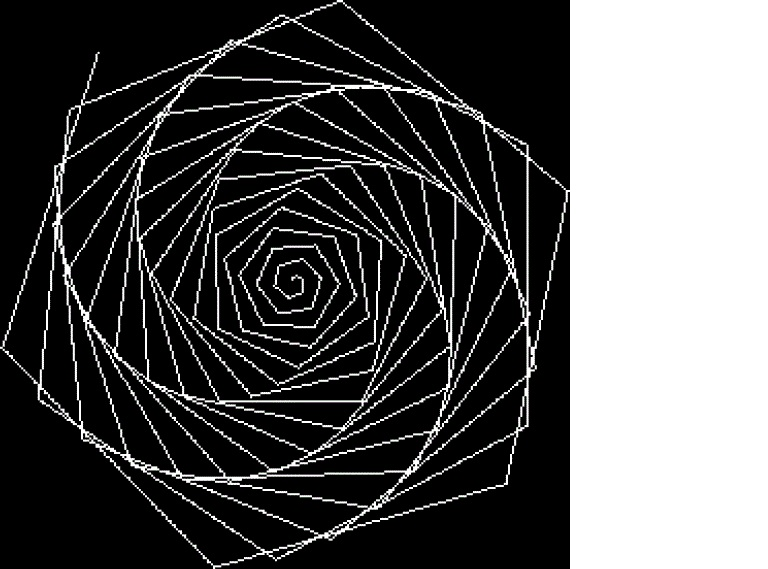
\includegraphics[width=5in]{../Pictures/spiral.jpg}
\end{center}

\subsection*{Nested Loops}
\begin{codesnippet}
{
   DO A FROM 1 TO 50 {
      FD A
      RT 30
      DO B FROM 1 TO 8 {
         SET C := A 5 / ;
         FD C
         RT 45
      }
   }
}
\end{codesnippet}
\begin{center}
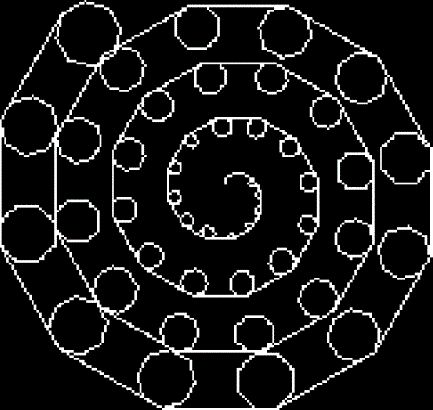
\includegraphics[width=5in]{../Pictures/nstdloop.jpg}
\end{center}

\subsection*{The Formal Grammar}
{\samepage
\begin{codesnippet}
<MAIN>        ::= "{" <INSTRCTLST>
<INSTRCTLST>  ::= <INSTRUCTION><INSTRCTLST> |
                  "}"
<INSTRUCTION> ::= <FD> |
                  <LT> |
                  <RT> |
                  <DO> |
                  <SET>
<FD>          ::= "FD" <VARNUM>
<LT>          ::= "LT" <VARNUM>
<RT>          ::= "RT" <VARNUM>
<DO>          ::= "DO" <VAR> "FROM" <VARNUM> "TO"
                  <VARNUM> "{" <INSTRCTLST>
<VAR>         ::= [A-Z]
<VARNUM>      ::= number | <VAR>
<SET>         ::= "SET" <VAR> ":=" <POLISH>
<POLISH>      ::= <OP> <POLISH> | <VARNUM> <POLISH> | ";"
<OP>          ::= "+" | "-" | "*" | "/"
\end{codesnippet}
}

